\subsection{问题一的模型建立与求解}
\label{sec:5.2}

本问按 \texttt{sec5\_q1.tex} 的三项任务组织：任务一建立唯一的文档与领域质量口径；任务二在评分之后诊断指标与来源之间的分歧；任务三把质量桥接到 17 个训练域、建立配比—损失模型并选出推荐配比，输出 P1 接口。三项共用同一套冻结参数，任务一与任务二的产物进入任务三与后续问题。

\subsubsection{任务一：数据质量评估}
\label{sec:5.2.1}

A1 的 22 个原始字段按输出形态展开为 25 项：4 个 \texttt{modernbert\_*} 六档 logits 各取 softmax 后的期望分；\texttt{qurater} 拆为四维；\texttt{ad\_en}、\texttt{fluency\_en} 取标签 1 的概率（\texttt{ad\_en} 的标签 1 表示无广告）；\texttt{fineweb\_edu} 取单元素值；3 个 DSIR 与 11 个 \texttt{rps\_*} 取原标量。词数、句数、平均词长与词熵按 A1 域内中位数转为适宜区间型 $-|h_j(x)-m_{dj}|$；正向指标保留、负向指标取负；重尾非负值按规则取 $\log(1+x)$。三个 DSIR 分量先除以 $\max(\mathrm{word\_count},1)$，再在 A1 各域内以 $\log(1+\mathrm{word\_count})$ 拟合带截距 OLS 并使用残差；A2/A3 复用 A1 的回归系数。各域各指标用 A1 的 1\%/99\% 分位缩尾，再按 A1 端点 Min–Max 归一到 $z_j(x)\in[0,1]$，缺失值用 A1 同域同指标标准化中位数填补。

长度校正的效果：A1 七域$\times$三 DSIR 的词数 Spearman 绝对相关中位数由原量 $0.957$ 降至除词数后的 $0.599$、再降至残差化后的 $0.095$，逐项见 \texttt{T2\_dsir\_length\_diagnostic.csv}。book 域剩余相关最高（$|\rho|=0.503$），提示该域分数仍可能受长度影响。这是与长度混杂有关的测量假设，不表示相关下降即去掉了无用信息。

\textbf{唯一主质量口径：CRITIC 加权 Huber 中心。} 在 A1 的标准化矩阵上，以 CRITIC 的离散度与指标间非冗余性确定固定权重\cite{critic}：

\begin{equation*}
C_j=s_j\sum_{k=1}^{25}(1-r_{jk}),\qquad w_j=\frac{C_j}{\sum_kC_k},\qquad \sum_j w_j=1 .
\end{equation*}

文档主质量分取加权 Huber 中心\cite{huber}

\begin{equation*}
Q(x)=\arg\min_{q\in[0,1]}\sum_{j=1}^{25}w_j\rho_\delta\bigl(z_j(x)-q\bigr),\qquad
\rho_\delta(u)=\begin{cases}\tfrac12u^2,&|u|\le\delta,\\ \delta(|u|-\tfrac12\delta),&|u|>\delta,\end{cases}
\end{equation*}

由导数方程 $\sum_jw_j\operatorname{clip}(q-z_j,-\delta,\delta)=0$ 在 $[0,1]$ 上二分求解。$\delta$ 只由 A1 确定：取每篇的加权指标中位数 $m_x$、加权 MAD $a_x=\operatorname{wmedian}_j|z_j-m_x|$，再取 $\delta=1.345\times1.4826\times\operatorname{median}_{x\in A1}a_x$，得 $\delta=0.4034907036619329$（1.4826 为正态尺度校正，1.345 为经典 Huber 效率常数）。这是一条不依赖质量真值与下游损失、也不依赖冲突类型的 A1 尺度规则，A2/A3 复用同一数值。25 项 CRITIC 权重逐项见 \texttt{T2\_critic\_weights.csv}（最小 \texttt{fineweb\_edu} 0.0359，最大 \texttt{modernbert\_professionalism} 0.0671），$\delta$ 的确定过程见 \texttt{T2\_delta\_selection.csv}。所有 A1 参数（方向、缩尾端点、Min–Max 端点、填补值、权重、$\delta$）一经确定即冻结，A2/A3 只应用、不重估。

对照口径 $Q_{\rm mean}=\sum_jw_jz_j$（同权重算术均值）、PCA 与 TOPSIS 只用于方法一致性比较：A1 主分与三者的 Spearman 分别为 $0.9936$、$0.8166$、$0.9588$（\texttt{T2\_method\_agreement.csv}）。这些是方法一致性，不是独立质量标签验证。极端指标扰动：逐篇剔除距加权中位数最远的一个指标后，极端程度最高 10\% 的文档（5,123 篇）中，主分的绝对变动中位数为 $0.0260$（P90 为 $0.0340$），算术均值为 $0.0374$（P90 为 $0.0488$），即主分对同一扰动的典型变动约小 30\%（\texttt{T2\_extreme\_influence.csv}）。该实验只覆盖"删除最偏离一项"，不覆盖全部异常模式。

\textbf{质量分求解。} 25 项标准化矩阵在 A1 上一次算出，然后在 A2/A3 上只做前向应用；主分按导数方程二分求根，权重与 $\delta$ 随之冻结。

\textbf{求解设置与复现。} 问题一为纯 NumPy/Pandas 实现（不依赖 SciPy 或 scikit-learn），运行环境为 Python 3.12.13、NumPy 2.4.4、pandas 3.0.2；标准运行顺序为 \texttt{q1\_01\_extract.py} $\to$ \texttt{q1\_02\_quality.py} $\to$ \texttt{q1\_03\_conflict.py}、\texttt{q1\_04\_bridge.py} $\to$ \texttt{q1\_05\_mixture.py} $\to$ \texttt{q1\_06\_scale.py}、\texttt{q1\_07\_optimal.py} $\to$ \texttt{q1\_08\_audit.py}，本轮全链耗时约 5 分钟（其中桥接约 160 秒）。随机种子在质量评分、桥接、配比拟合与候选搜索中分别固定为 $2026$、$42$、$2026$、$1234$（另：A1 域内聚类子步用 $42$，冲突抽样子步用 $0$ 与 $7$，来源一致性实验用 $42$）。关键求解参数：质量中心的导数二分固定 28 次；配比 Huber 回归以最小二乘初始化，标准化残差阈值 $1.35$，IRLS 最多 50 次、以最大系数变化小于 $10^{-8}$ 停止；桥接按域分层五折、只在训练折估计特征标准化参数，GBDT 用深度 1 树桩与学习率 $0.06$，五折比较用 250 棵、最终拟合用 300 棵；配比对照的 GBDT 用五折交叉验证在 $\{$学习率$\}\times\{$树数$\}$ 网格上选参。以上参数与脚本路径见 \texttt{src/code\_q1/q1\_00\_common.py} 及各 Step 脚本。树数与候选数是预设计算上限，不应误写为已证明的优化收敛。

\textbf{主质量分与领域质量。} A1 七个领域的 CRITIC 加权 Huber 主分中位数由高到低为：arxiv $0.7707$、commoncrawl $0.6761$、stackexchange $0.6600$、c4 $0.6545$、book $0.6313$、github $0.6172$、wikipedia $0.5991$（\texttt{T2\_domain\_quality.csv}，图~\ref{fig:F2_domain_quality_box}）。图~\ref{fig:F2_domain_quality_box} 显示七域主分的分布区间，可见 arxiv 与 wikipedia 的域内分布几乎不重叠，领域间差异大于多数域内差异，这是按域建尺度、再按域汇总的必要性依据。领域分取文档中位数，并以 2,000 次文档 bootstrap 给出条件区间；book 域仅 171 篇，域内细分比例须谨慎使用。

\begin{figure}[H]
\centering
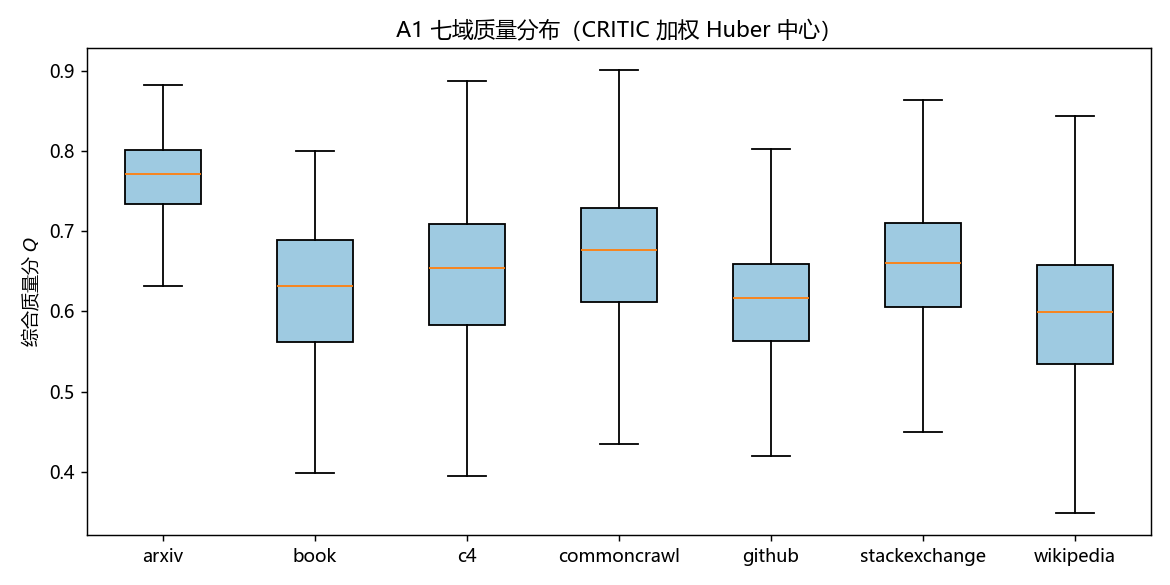
\includegraphics[width=\textwidth]{figs/q1_F2_domain_quality_box.png}
\caption{A1 七个领域的 CRITIC 加权 Huber 主分分布}
\label{fig:F2_domain_quality_box}
\end{figure}

扩展集的表现：A2 的 arxiv 中位数为 $0.7697$，对应 A1 子集为 $0.7707$；A3 的 github 中位数为 $0.6158$，对应 A1 子集为 $0.6172$；两组 KS 检验的 $p$ 值为 $0.313$ 与 $0.220$（\texttt{T2\_sampling\_check.csv}）。$p$ 值只能说明在冻结管线下未检出明显分布差异，不能证明抽样完全无偏或分数具有独立准确性。

方法一致性与扰动稳健性：主分与同权重算术均值、PCA、TOPSIS 的文档排序 Spearman 分别为 $0.9936$、$0.8166$、$0.9588$（\texttt{T2\_method\_agreement.csv}）；删除最偏离一项指标后，极端程度最高 10\% 文档的主分绝对变动中位数为 $0.0260$、P90 为 $0.0340$，算术均值对应为 $0.0374$ 与 $0.0488$（\texttt{T2\_extreme\_influence.csv}）。这些数值是 $[0,1]$ 评分尺度上的绝对变动，即 2.6 与 3.7 个百分点，\textbf{不是质量提升率}；对同一项极端指标扰动，Huber 的典型变动约小 30\%，这是把 Huber 中心作为主分的稳健性依据，但仍不能替代人工质量标签。

\textbf{检验与边界。} 本任务的结果分三层检查（设计与结论汇总见 \ref{sec:6.1}）：A2/A3 是\textbf{冻结评分的扩展检验}，KS 的 $p$ 值只说明在冻结管线下未检出明显分布差异，不等于抽样无偏或分数准确；主分与算术均值、PCA、TOPSIS 的秩相关是\textbf{方法一致性}，不是与人工标签的吻合度；删除最偏离一项指标的扰动只覆盖一种异常模式。因此本任务不报告质量准确率，只报告排序口径、稳健性与适用边界。

\subsubsection{任务二：质量指标冲突的诊断与消解}
\label{sec:5.2.2}

诊断在 \ref{sec:5.2.1} 的主分之后进行，\textbf{不参与 CRITIC 权重、Huber 中心、桥接标签或任何 P1 接口}。按指标生成机制固定六个来源：RPS（11 项）、DSIR（3 项）、轻量分类器（2 项）、FineWeb-Edu（1 项）\cite{fineweb}、QuRating（4 项）、ModernBERT（4 项），每项指标恰好归属一处。对 A1 每个领域、每项指标保存标准化分的完整经验分布 $F_{dj}^{A1}$，文档的指标排名取 $r_j(x)=F_{dj}^{A1,\mathrm{mid}}(z_j(x))$（同值取中秩）；A2/A3 按对应领域查同一份冻结分布，不重新排名、不重估阈值，未见领域报错而不临时拟合。

来源中心 $m_s(x)=\operatorname{median}_{j\in I_s}r_j(x)$ 经 A1 同域同来源的中心分布转成 $u_s(x)$，六来源分歧度为

\begin{equation*}
B(x)=\max_{s=1,\dots,6}u_s(x)-\min_{s=1,\dots,6}u_s(x).
\end{equation*}

阈值取 A1 每域 $B$ 的第 95 百分位（同域同来源跨度与最大留一偏离同样取 P95），并报告 P90/P95/P97.5 与高低端立场 10\%/20\%/25\% 的敏感性。第 95 百分位使 A1 每域约 5\% 的文档入选，这是\textbf{预先选定的筛查预算，不是真实冲突的发现率}。仅当 $B$ 超阈值、且高端（$u_s\ge0.8$）与低端（$u_s\le0.2$）各有至少两个来源支持时，才记为"多来源对立候选"；仅一侧或多个来源不足时单列为稀疏来源对立。另用来源内跨度 $P_{90}(r_j)-P_{10}(r_j)$ 与逐指标留一中位数偏离 $e_j$ 识别孤立指标，单独记为"单指标独有候选"，不与来源间候选相加。来源配对方向按每篇文档的高端$\times$低端组合平均分配总权重 1。

\textbf{诊断求解。} 诊断阶段对 A1 每域、每指标保存有序经验分布作为参照，对 A2/A3 查表排名；A1 固定随机抽样 8,000 篇计算各来源 Kendall $W$；阈值取 A1 同域分位数，逐集逐域输出候选比例、重合度与方向份额。

\textbf{六来源分歧诊断的结果。}

\begin{table}[H]
\centering\small
\caption{三个数据集上的六来源诊断候选规模（数据源：\texttt{T3\_six\_source\_candidate\_summary.csv}）}
\label{tab:q1conflict}
\begin{tabularx}{\textwidth}{@{}lccc@{}}
\toprule
候选类型 & A1：51,230 篇 & A2：17,523 篇 & A3：203,752 篇 \\
\midrule
来源间高分歧 & 2,561（5.00\%） & 829（4.73\%） & 10,167（4.99\%） \\
其中多来源对立 & 695（1.36\%） & 277（1.58\%） & 3,598（1.77\%） \\
其中稀疏来源对立 & 1,866（3.64\%） & 552（3.15\%） & 6,569（3.22\%） \\
单指标独有 & 2,879（5.62\%） & 709（4.05\%） & 8,606（4.22\%） \\
\bottomrule
\end{tabularx}
\end{table}

表中百分比的分母均为该数据集的全部文档数。A1 的约 5\% 来自预设的 P95 筛查预算，\textbf{不能称为测得的真实冲突率}；多来源对立与稀疏来源对立互斥，单指标独有候选是另一类筛查，\textbf{不与来源间候选相加为"总冲突率"}。

来源内部一致性差异明显：A1 的 Kendall $W$ 依次为 RPS $0.140$、DSIR $0.967$、轻量分类器 $0.691$、QuRating $0.675$、ModernBERT $0.579$，FineWeb-Edu 只有一项指标故不定义；A1 文档内指标排名 $P_{90}-P_{10}$ 的中位数 RPS 为 $0.625$，DSIR 为 $0.037$，QuRating 为 $0.277$，ModernBERT 为 $0.315$；A1 有 $69.45\%$ 的文档在 RPS 内部同时存在低于 20\% 与高于 80\% 的指标（\texttt{T3\_six\_source\_consistency.csv}、\texttt{T3\_source\_internal.csv}，图~\ref{fig:F3_source_internal}）。图~\ref{fig:F3_source_internal}显示六来源内部跨度的量级差异，说明同一"规则型"来源内部就可能给出相反意见，因此把 11 项 RPS 压成一个中位数会掩盖意见分裂。这表示不同规则统计量给出相反的相对排序，\textbf{不能直接判为测量错误或真实质量矛盾}。

来源间的对立方向：A1 与 A3 的最高加权方向均为"RPS 高$\times$FineWeb-Edu 低"，份额为 $8.03\%$ 与 $13.03\%$；A2 为"ModernBERT 高$\times$FineWeb-Edu 低"，$9.89\%$（分母均为该集的六来源高分歧候选，且每篇文档的来源对总权重为 1，\texttt{T3\_source\_opposition\_pairs.csv}，图~\ref{fig:F3_source_opposition}）。映回旧四组时，原"模型评分器"组内部的新方向在三集占 $4.44\%$、$19.33\%$、$3.68\%$（\texttt{T3\_direction\_stability.csv}），即旧的四组口径无法显示这一类来源之间的分歧。

阈值与旧法对照：固定高低端立场为两端 20\% 时，A1 的 $B$ 阈值取 P90/P95/P97.5 对应候选比例约 $10.00\%/5.00\%/2.50\%$，A2 为 $9.19\%/4.73\%/2.00\%$，A3 为 $9.74\%/4.99\%/2.44\%$（\texttt{T3\_threshold\_sensitivity.csv}，图~\ref{fig:F3_threshold_sensitivity}）。历史四组口径的候选比例为 $19.08\%/24.52\%/23.28\%$，与六来源候选集合的 Jaccard 为 $0.188/0.130/0.155$；按 A1 各域前 5\% 配平预算后旧四组选出 $5.00\%/4.42\%/4.78\%$，Jaccard 提高至 $0.324/0.283/0.259$、Kappa 为 $0.463/0.415/0.381$（\texttt{T3\_legacy\_stability.csv}，图~\ref{fig:F3_legacy_overlap}、图~\ref{fig:F3_matched_overlap}）。Kappa \textbf{不是准确率}；历史阈值与新 P95 的选择预算不同，这组重合度不能单独解释为分组效果。

来源一致性加权对照实验：以各来源 Kendall $W$ 作先验可靠性乘数调整 CRITIC 权重（$\tilde w_j=w_j\cdot W_{s(j)}$，其余环节不变），得到的实验分 $Q_{\rm v2}$ 与主分在 A1/A2/A3 的全局 Spearman 为 $0.9547/0.9207/0.9395$，A1 七域的中位数排序与主分完全一致（\texttt{T3\_Q\_v2\_summary.csv}、\texttt{T3\_Q\_v2\_weight\_comparison.csv}，图~\ref{fig:F3_Q_v2_domain_median}）。Spearman 只衡量排序相似度，\textbf{不是 $Q_{\rm v2}$ 更准确的证据}；该分不替换主质量口径，也不写入任何 P1 接口。

\textbf{检验与边界。} 三集复现的是\textbf{诊断结构}而不是逐篇冲突类型：候选比例稳定（$5.00\%/4.73\%/4.99\%$），但最高加权对立方向在 A2 与 A1/A3 不同；Jaccard 与 Kappa 只用于比较两套候选集合的重合度（\textbf{Kappa 不是准确率}）；阈值敏感性反映的是人工复核工作量的变化。诊断层产物不参与 CRITIC 权重、Huber 中心、桥接标签或任何 P1 接口，筛查预算也不解释为真实冲突率。

\subsubsection{任务三：领域配比、语料质量与损失}
\label{sec:5.2.3}

\textbf{桥接到 17 个配比域。} A16 的 17 个配比域中 3 个为 direct、3 个为 near\_direct、11 个为 inferred。对 11 个无直接质量信号的域，从 A1/A18 原文各自复算 11 项同名近似规则特征 $\Phi(text)$（不保证逐位复现附件 \texttt{rps\_*}）。在 A1 的 21,590 篇原文上以 \ref{sec:5.2.1} 的同一 $Q(x)$ 为标签，按领域分层五折比较 Ridge 与 GBDT（每折的特征均值与标准差仅用训练折估计，避免折间泄漏），选较优者对 A18 的 31,340 篇预测并逐域聚合。六个 direct/near\_direct 映射域的 $Q_{\rm final}$ 取对应 A1 质量域主分中位数，$CI_{\rm lo/hi}$ 同取该 A1 域主分 bootstrap；11 个 inferred 域取 A18 预测中位数与文档 bootstrap。$Q_{\rm tokenw}$ 按最终来源取值。语料质量按份额聚合：

\begin{equation*}
Q(\bp)=\sum_{i=1}^{17}p_iQ_i,\qquad p_i\ge0,\quad\sum_ip_i=1 .
\end{equation*}

桥接模型的五折表现与六个映射域的一致性见本小节下文；区间口径与点估计必须同源，不能用 A1 点估计配 A18 预测区间，17 域逐行断言点估计落在同源区间内。

\textbf{桥接求解。} A1 的 21,590 篇按域分层五折，折内标准化参数只用训练折估计；五折比较 Ridge 与 GBDT 后取较优者用全部训练子集拟合，再对 A18 的 31,340 篇预测并逐域取中位数与文档 bootstrap 区间。

\textbf{从文档质量到 17 域质量。} 桥接模型在 A1 上的分层五折 $R^2$ 均值为 $0.4106$（Ridge 为 $0.3415$，\texttt{T4\_calibration\_cv.csv}）；六个可映射域的预测与 A1 主分的 Pearson 为 $0.6571$、Spearman 为 $0.7714$、MAE 为 $0.0365$，但 $n=6$（\texttt{T4\_bridge\_validation.csv}）。17 域 $Q_{\rm final}$ 最高为 arxiv $0.7707$、最低为 dm\_mathematics $0.5087$（\texttt{T4\_bridge\_17domains.csv}，图~\ref{fig:F4_bridge_17domains}）。图~\ref{fig:F4_bridge_17domains} 显示 17 个域的质量分与按来源构造的条件区间，六个 direct/near\_direct 域的点估计与区间同取 A1 主分，11 个 inferred 域取 A18 预测中位数与文档 bootstrap。使用边界有三条：映射域区间以 A16 映射成立为条件，尤其不覆盖 near\_direct 的映射偏差；inferred 区间只反映\textbf{给定桥接模型}下的文档抽样变动，不涵盖模型选择与跨域偏差；ubuntu\_irc（16 篇）与 philpapers（63 篇）须低置信使用。桥接 $R^2$ 与六域一致性\textbf{都不是独立质量准确率}。

\begin{figure}[H]
\centering
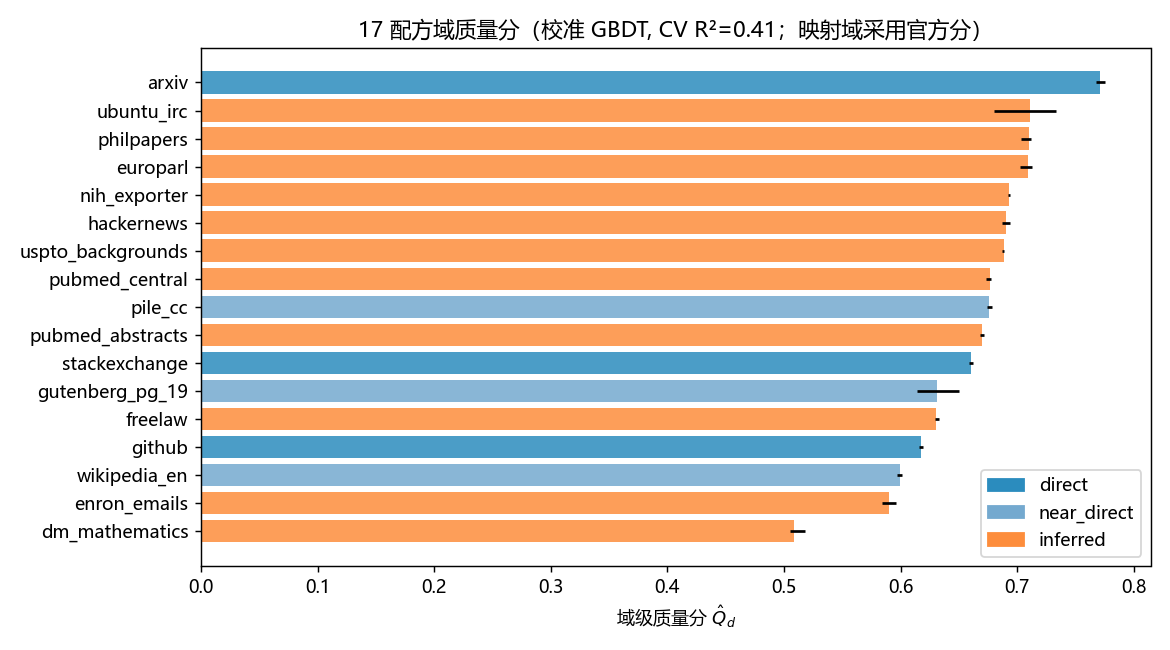
\includegraphics[width=\textwidth]{figs/q1_F4_bridge_17domains.png}
\caption{17 个配比域的质量分与条件区间}
\label{fig:F4_bridge_17domains}
\end{figure}

\textbf{配比—损失模型与迁移结构。} A4/A5 按 \texttt{index} 连接后作 1M 配比训练集（非正份额替换为 $10^{-4}$ 并重新闭合）。配比份额受闭合约束，直接回归会有闭合效应，故作中心对数比变换

\begin{equation*}
\xi_i(\bp)=\log p_i-\frac1{17}\sum_{k=1}^{17}\log p_k,\qquad
\log L_v=b_v+\sum_{i=1}^{17}\beta_{vi}\xi_i(\bp)+\varepsilon_v,
\end{equation*}

对 13 个验证域分别拟合 Huber 回归\cite{aitchison,regmix}，这是\textbf{唯一主模型}；原始份额 OLS 检验变换的作用，深度 1 的树桩 GBDT 检验线性形式是否漏掉重要非线性。在均匀配比处把系数投影到单纯形切空间，得 $17\times13$ 迁移矩阵 $T_{iv}=17(\beta_{vi}-\bar\beta_v)$，其中 $\bar\beta_v=17^{-1}\sum_i\beta_{vi}$。另拟合质量交互项 $\lambda_v\sum_ip_i(1-Q_{i,\rm final})$，用 400 次案例 bootstrap 给区间并在 A6/A7 检查预测。

GBDT 的树数与学习率\textbf{只在 A4/A5 内部}用五折交叉验证选定：折号由固定种子随机置换得到，网格为学习率 $\{0.03,0.06,0.12,0.25\}\times$ 树数 $\{100,250,500,1000\}$，准则为 13 域留折 $\ln L$ RMSE 的均值，选定后用全部 512 组重拟合；A6–A11 不参与选参。GBDT 在 A4/A5 上按等权 Loss 另选一个 $\bp^*$ 作交叉评估，用于检验线性模型的最优配比是否稳健，\textbf{不作主模型}（理由是可解释性与接口一致性，而非预测更差）。

\textbf{配比与跨尺度求解。} clr+Huber 回归对 13 个验证域分别拟合；迁移矩阵由 clr 链式法则折算到单纯形切空间；GBDT 选参只在 A4/A5 内部完成；尺度修正的 $\rho_v,\kappa$ 只由 A4/A5 与 A8/A9 闭式确定；1M 留出、60M、1B 与估算表全部用冻结模型评估，不做二次拟合。

\textbf{配比—损失关系与迁移结构。} 在 A6/A7 的 1M 留出（256 组）上，13 域平均逐域 $R^2$ 为 clr+Huber $0.772$、原始份额 OLS $0.654$、GBDT（选参后）$0.923$；目标 Spearman 为 GBDT $0.942$、线性 $0.523$；但 13 域等权目标 $R^2$ 上裸 OLS 的 $0.418$ 高于 clr+Huber 的 $0.260$（\texttt{T5\_model\_comparison.csv}）。因此本文保留 clr+Huber 解释局部迁移效应，同时以留出目标表现更好的 GBDT 作交叉评估，\textbf{不声称 clr 在所有目标上都更优}。GBDT 的五折选参结果为 1,000 棵、学习率 $0.12$，留折 $\ln L$ RMSE 为 $0.0421$；学习率 $0.25$ 在 500 棵时为 $0.0422$、到 1,000 棵回升至 $0.0426$，说明最优点在网格内部，且最优点附近曲线很平（\texttt{T5\_gbdt\_cv.csv}）。质量交互项在 13 域中仅 6 域的系数区间不含零，且系数有正有负，只能说明质量与配比损失存在混杂关联，\textbf{不构成质量因果效应}（\texttt{T5\_lambda\_interaction.csv}）。17$\times$13 迁移矩阵的各域主对角元均为负（\texttt{T5\_transfer\_matrix.csv}，图~\ref{fig:F5_transfer_matrix}），图~\ref{fig:F5_transfer_matrix} 显示各验证域对训练域份额的局部敏感度结构。

\begin{figure}[H]
\centering
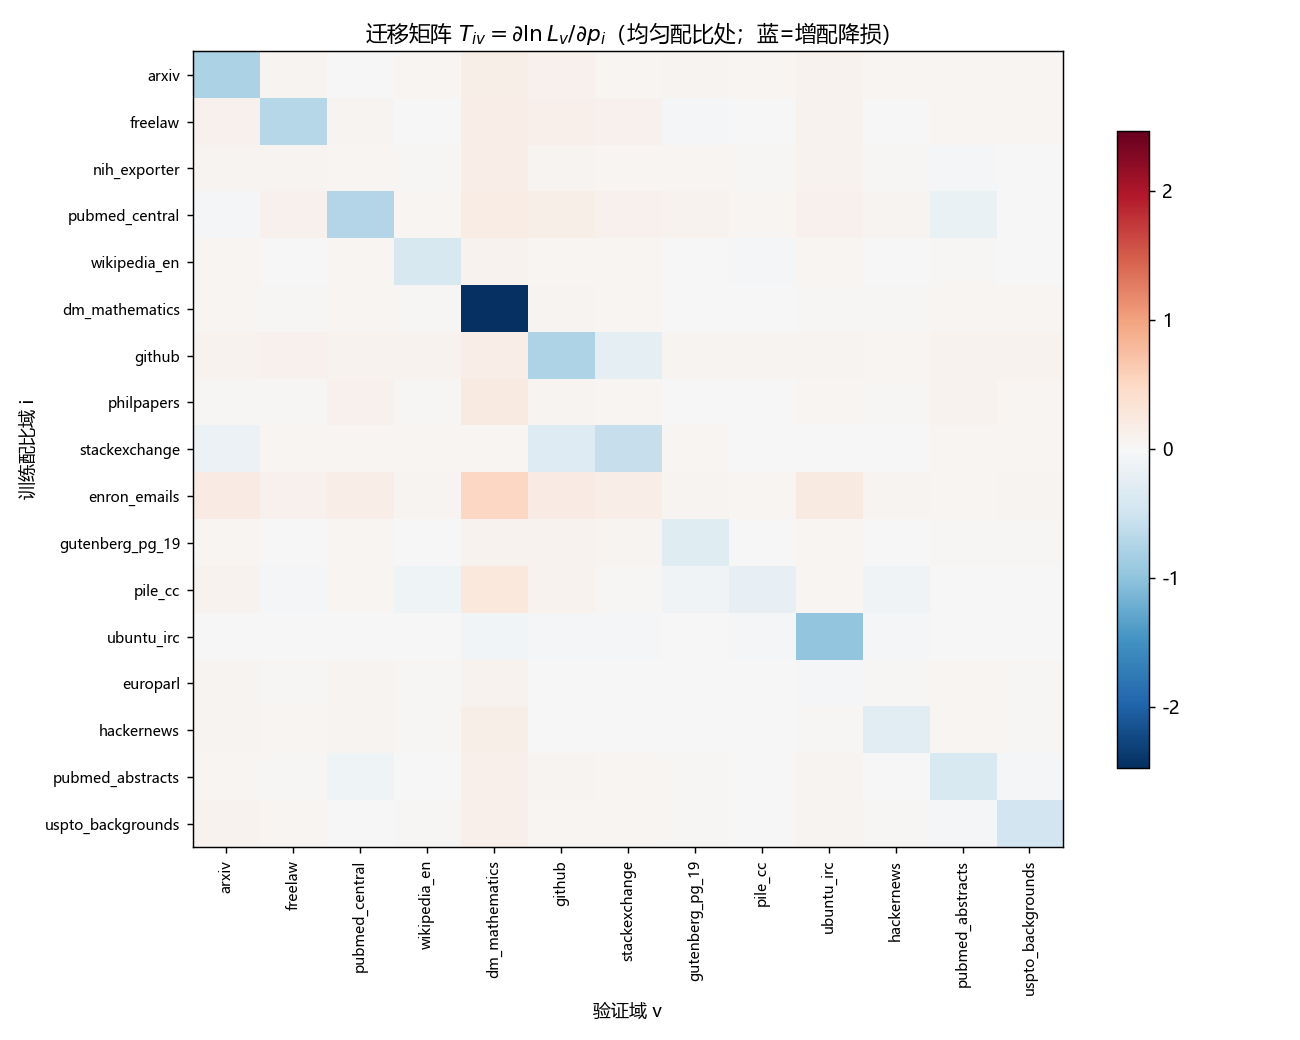
\includegraphics[width=0.92\textwidth]{figs/q1_F5_transfer_matrix.png}
\caption{$17\times13$ 迁移矩阵：各验证域对训练域份额的局部敏感度}
\label{fig:F5_transfer_matrix}
\end{figure}

\textbf{跨尺度检验与尺度修正。} 冻结检验：在 A4/A5 上拟合后冻结线性模型与 GBDT，直接预测 1M 留出、60M 与 1B，报告绝对误差与排序。尺度修正保持 1M 配比系数 $\boldsymbol\beta_v^{\rm 1M}$ 不变，记 $g_v(\bp)=\boldsymbol\beta_v^{\rm 1M}\cdot\operatorname{clr}(\bp)$、$t=\ln(N/10^6)$：

\begin{equation*}
\ln L_v(\bp,N)=\underbrace{b_v^{\rm 1M}+\rho_vt}_{\text{截距漂移}}+\underbrace{(1+\kappa t)}_{s(N)}\,g_v(\bp).
\end{equation*}

$b_v^{\rm 1M}$ 与 $s(10^6)=1$ 来自 A4/A5；在 A8/A9（60M）上求汇总斜率 $s(60{\rm M})=\sum_v\operatorname{cov}(y_v,g_v)/\sum_v\operatorname{var}(y_v)$ 与逐域截距 $b_v(60{\rm M})=\bar y_v-s(60{\rm M})\bar g_v$，由两点闭式得到 13 个 $\rho_v$ 与 1 个共同 $\kappa$。\textbf{A10/A11（1B，各 64 行）不参与任何估计}，只用于比较冻结模型、仅截距修正与截距加缩放修正三种口径；另报"1B 同集拟合"作为该函数形式的误差下界参照，不作结论。估算表 A12–A15 是 10B/70B 的估算或外推 Loss，与冻结模型、尺度修正模型和同配比 1M 实测 Loss 并列对照，\textbf{不是观测}。

\textbf{跨尺度检验的结果。} 冻结 1M 模型的等权目标 Spearman 在 1M 留出/60M/1B 上为线性 $0.523/0.467/0.677$、GBDT $0.942/0.905/0.761$；GBDT 的目标 MAE 为 $0.078/1.466/2.713$（\texttt{T6\_cross\_scale\_validation.csv}、\texttt{T6\_gbdt\_cross\_scale.csv}，图~\ref{fig:F6_rank_decay}）。图~\ref{fig:F6_rank_decay} 显示冻结模型在三档规模上的排序保持度：排序信息基本保持，但 60M/1B 的绝对 Loss 有大幅平移（$R^2$ 为负），\textbf{排序部分保持不等于损失水平可直接迁移}。1B 只有 64 组，Spearman 的抽样误差约 $\pm0.1$，GBDT 在 1B 的领先幅度只能算中等证据。

\begin{figure}[H]
\centering
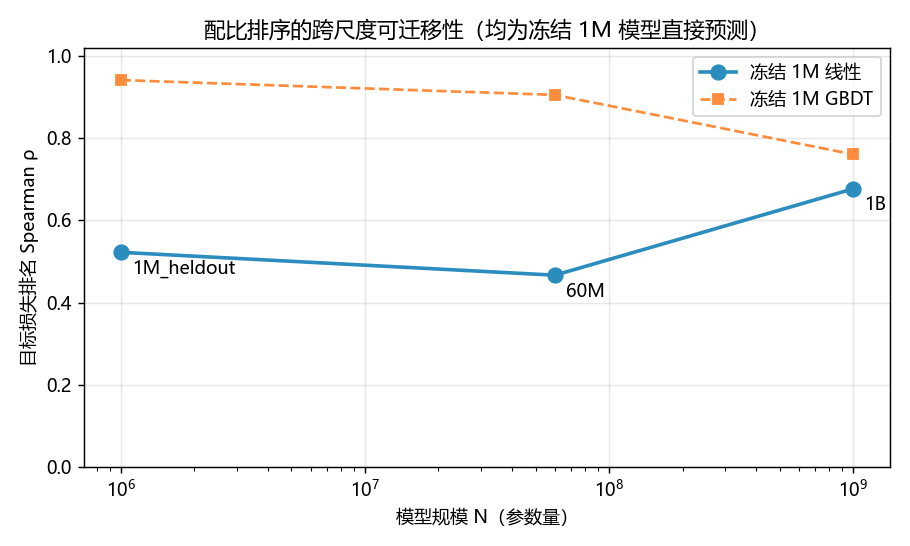
\includegraphics[width=\textwidth]{figs/q1_F6_rank_decay.png}
\caption{冻结 1M 配比模型在 1M 留出、60M 与 1B 上的排序保持度}
\label{fig:F6_rank_decay}
\end{figure}

尺度修正由 1M 训练与 60M 标定给出 $s(60{\rm M})=0.913$、$\kappa=-0.0212$，外推到 1B 为 $s(1{\rm B})=0.854$（\texttt{T6\_scale\_correction\_params.csv}，图~\ref{fig:F6_scale_correction}）。

\begin{figure}[H]
\centering
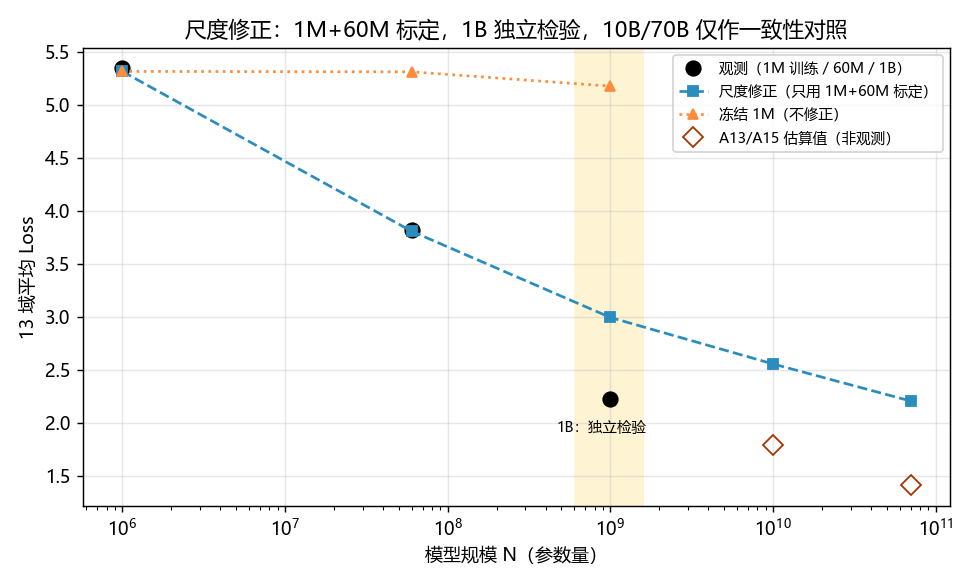
\includegraphics[width=\textwidth]{figs/q1_F6_scale_correction.png}
\caption{尺度修正前后的绝对 Loss 对照（1M＋60M 标定，1B 独立检验）}
\label{fig:F6_scale_correction}
\end{figure}

\begin{table}[H]
\centering\footnotesize
\caption{给出 1B 独立检验（A10/A11，各 64 组，不参与任何估计）的结果（数据源：\texttt{T6\_scale\_correction.csv}）}
\label{tab:q1scale1b}
\begin{tabularx}{\textwidth}{@{}X r r r r r@{}}
\toprule
1B 口径 & 逐域 MAE 均值 & 目标 MAE & 逐域 $R^2$ 均值 & 目标 Spearman & 平均预测 Loss \\
\midrule
冻结 1M & 2.953 & 2.953 & -604.7 & 0.677 & 5.178 \\
仅截距修正 & 0.770 & 0.768 & -33.4 & 0.712 & 2.994 \\
截距＋缩放修正 & 0.771 & 0.771 & -35.3 & 0.713 & 2.997 \\
1B 同集拟合（误差下界参照，不作结论） & 0.082 & 0.029 & 0.624 & 0.702 & 2.222 \\
\bottomrule
\end{tabularx}
\end{table}

1B 的观测平均 Loss 为 $2.226$。由此得到三条结论：\textbf{方向对、幅度不足}——修正把 1B 绝对误差降低约 74\%（$2.95\to0.77$），但平均预测 $2.99$ 仍明显高于观测 $2.23$，1M$\to$60M 每单位 $\ln N$ 的 Loss 降幅约 $0.08$、60M$\to$1B 段约 $0.19$，两档规模的对数线性外推无法捕捉该曲率；\textbf{效应缩放的外推偏差更大}（预测 $s(1{\rm B})=0.854$，同集拟合为 $0.612$，加缩放项对 MAE 没有帮助，下游若用 1M 配比效应推断大尺度收益应以 $0.61$ 为 1B 的实测幅度）；\textbf{误差来源是水平外推而非配比结构}（同一函数形式直接在 1B 上拟合时 MAE 仅 $0.08$）。在 60M 标定集上（同集，不作检验），修正把逐域 MAE 从 $1.490$ 降到 $0.206$（仅截距）/ $0.208$（截距＋缩放）。

跨尺度校准接口（仅评估）：冻结 1M 系数的汇总斜率在 1M 训练/1M 留出/60M/1B 上为 $1.004/0.995/0.913/0.612$，观测平均 Loss 为 $5.345/5.282/3.823/2.226$（\texttt{interface/P1\_scale\_calibration.csv}，\texttt{T6\_scale\_correction.csv}）。配比效应的方向跨尺度保持，幅度在 1B 缩到约六成。

估算表 A12–A15（\textbf{外推/估算，非观测}）：在同样 63 组配比上，冻结线性预测的 10B/70B 目标 Spearman 为 $-0.532/-0.588$、逐域 MAE 为 $3.53/3.91$，尺度修正后为 $-0.537/-0.576$ 与 $0.86/0.88$；估算表本身的平均 Loss 为 $1.797$（10B）、$1.415$（70B），低于修正模型的外推，方向与 1B 上"实际下降快于两档外推"一致（\texttt{T6\_extrapolation.csv}）。估算表的目标 Loss 排序与 1M 实测几乎相反（同配比从 1M 到 60M 的实测排序逐域 Spearman $\ge0.98$，\texttt{T6\_domain\_stability\_rank.csv}），因此估算表隐含的"大尺度排序反转"\textbf{没有观测支持}，只作为稳健性讨论的反例。注意 A12/A14 的 63 组配比逐行等于 A4 的子集（代码断言），冻结模型在这些配比上并非样本外；A13/A15 本身由三尺度幂律外推生成，与修正模型的接近\textbf{只是一致性对照，不构成独立验证}。

\textbf{候选最优配比。} 以 A4 平均配比为中心、四档浓度 Dirichlet 生成 99,996 个候选。主口径由线性 clr+Huber 模型在\textbf{信赖域}内选取：候选的 clr 向量到 A4 训练配比的马氏距离（协方差加 $10^{-3}I$ 岭）不超过训练配比自身距离的 95\% 分位，且每域份额不超过 A4 该域最大值。信赖域内分别按 13 域等权 Loss 与 pile\_cc Loss 取预测最优的前 100 个份额平均，得 \texttt{p\_star\_eqweight} 与 \texttt{p\_star\_pilecc}，并核对平均后的 $\bp^*$ 仍在信赖域内；GBDT 在同一信赖域内按等权 Loss 另选 \texttt{p\_star\_gbdt\_eqweight} 作稳健性对照，报告两者的全变差距离与交叉评估。不确定性有两项：固定线性 $\bp^*$ 的 200 次案例 bootstrap 重拟合收益分布，以及每次 bootstrap 在同一信赖域内重选 $\bp^*$ 与主 $\bp^*$ 的全变差距离分布。每个候选的 \texttt{Q\_domain} 从本轮 $Q_{\rm final}$ 按域名连接，$\bar Q=\sum_ip_iQ_i$。不加信赖域时线性模型会在远离训练分布的组合上给出不可信的低 Loss（前 100 个候选的马氏距离中位数约 $3.1\times10^4$，预测等权 Loss 中位数低至 $0.84$，而均匀配比为 $5.39$），故信赖域是本方案的建模选择而非数据结论。

\textbf{候选配比求解。} 99,996 个 Dirichlet 候选先按 clr 马氏距离与份额上限筛入信赖域，再按 13 域等权预测损失（或 pile\_cc 单域损失）取前 100 个份额平均；线性模型选主口径，GBDT 在同信赖域内另选作对照与交叉评估。

\textbf{推荐配比与配比加权质量。} 信赖域阈值取 clr 马氏距离 $21.85$（A4 训练配比距离的 95\% 分位），保留 46,168/99,996 个候选。

\begin{table}[H]
\centering\footnotesize
\caption{候选配比的对照（数据源：\texttt{T7\_pstar\_benchmark.csv}、\texttt{interface/P1\_p\_star.csv}）}
\label{tab:q1pstar}
\begin{tabularx}{\textwidth}{@{}p{2.7cm} r r r r r r@{}}
\toprule
配比 & \makecell{线性预测\\等权 Loss} & \makecell{GBDT 预测\\等权 Loss} & \makecell{线性\\评估收益} & \makecell{GBDT\\交叉评估收益} & 马氏距离 & $\bar Q$ \\
\midrule
$\bp^*$ 等权（线性，主口径） & 4.875 & 4.901 & 9.47\% & 9.47\% & 13.9 & 0.66241 \\
$\bp^*$ GBDT 对照 & 4.927 & 4.811 & 8.51\% & 11.12\% & 10.4 & 0.66297 \\
$\bp^*$ pile\_cc（线性） & 5.074 & 4.963 & 5.77\% & 8.31\% & 4.0 & 0.66393 \\
训练配比均值 & 5.198 & 5.177 & 3.48\% & 4.36\% & 0.5 & 0.66399 \\
均匀配比 & 5.385 & 5.413 & 0 & 0 & 2.7 & 0.66065 \\
\bottomrule
\end{tabularx}
\end{table}

表中收益的分母为\textbf{均匀配比的预测等权 Loss}（$5.385$），是 1M 代理模型在同一模型内的预测差异，\textbf{不是重新训练后的实测改善}。三点结论：两种模型选出的配比几乎相同（全变差距离 $0.0344$，GBDT 独立评估线性 $\bp^*$ 的收益为 $9.47\%$，与线性自评一致，故主口径改用线性不损失收益）；收益的不确定性为固定 $\bp^*$ 的 bootstrap 收益中位数 $9.54\%$、95\% 区间 $[7.82\%,11.16\%]$，每次重选 $\bp^*$ 与主 $\bp^*$ 的全变差中位数 $0.019$、P95 $0.027$（\texttt{T7\_gain\_ci.csv}，图~\ref{fig:F7_p_star}）；pile\_cc 口径较弱（按线性模型只把 pile\_cc Loss 从 $5.576$ 降到 $5.569$，GBDT 评估反而更高，只能称搜索候选）。图~\ref{fig:F7_p_star}显示两个目标口径下信赖域内候选的分布与主 $\bp^*$、均匀配比的位置。

\begin{figure}[H]
\centering
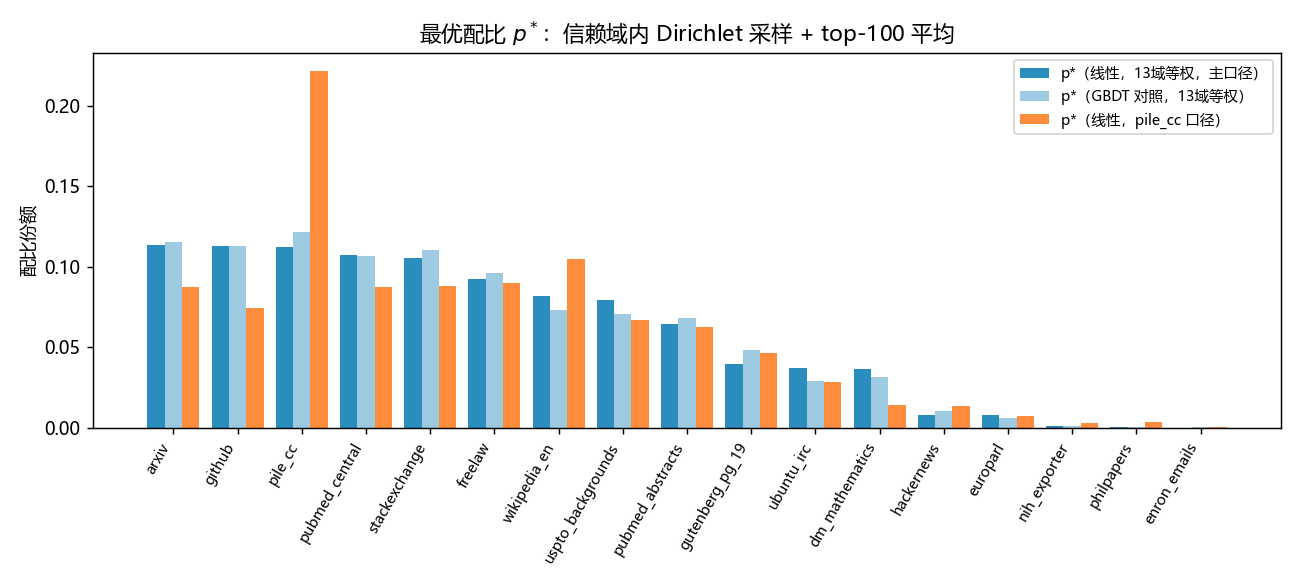
\includegraphics[width=\textwidth]{figs/q1_F7_p_star.png}
\caption{信赖域内候选配比的分布与推荐配比 $\bp^*$、均匀配比的位置}
\label{fig:F7_p_star}
\end{figure}

质量与训练边际价值在 17 域上的 Spearman 为 $-0.211$（\texttt{T7\_quality\_vs\_value.csv}，图~\ref{fig:F7_quality_vs_value}），说明单凭域质量分不能代替配比实验：质量高不等于该域的训练边际价值高。图~\ref{fig:F7_quality_vs_value}显示 17 域质量分与边际价值的散点关系，两轴方向相反但并非单调替代关系，\textbf{该相关性不是因果结论}。主 $\bp^*$ 的配比加权质量 $\bar Q(\bp^*)=0.6624116679870492$；训练配比均值处为 $0.6639855669942757$，均匀配比处为 $0.6606498405290009$（\texttt{interface/P1\_summary.json}）。注意候选配比的预测损失\textbf{不随 $Q$ 改变}：配比搜索只依赖配比与 Loss，质量分只改变 $\bar Q$ 的数值口径。

\begin{figure}[H]
\centering
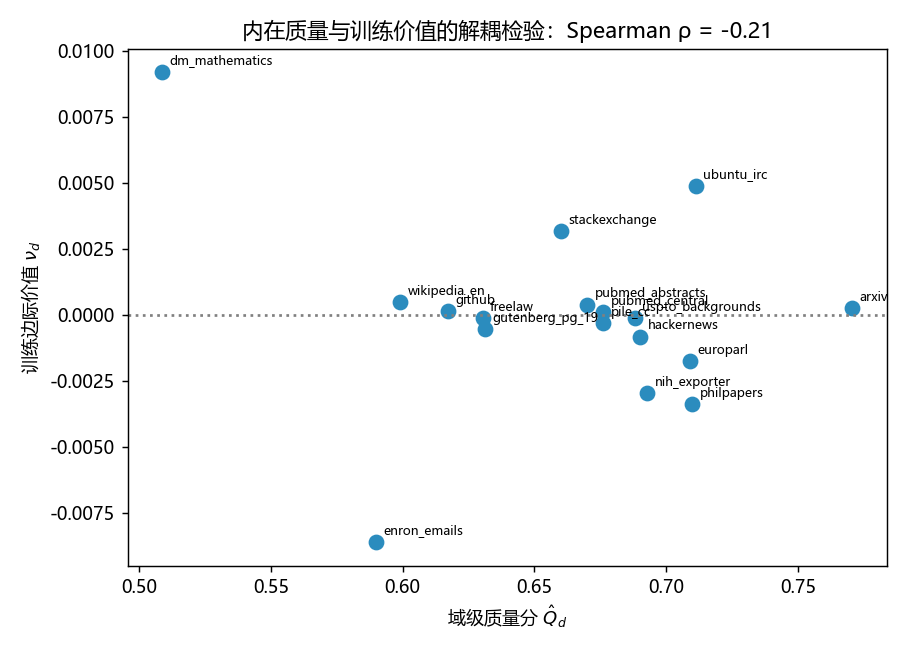
\includegraphics[width=0.78\textwidth]{figs/q1_F7_quality_vs_value.png}
\caption{17 域质量分与训练边际价值的散点关系}
\label{fig:F7_quality_vs_value}
\end{figure}

\textbf{检验与边界。} 本任务的检验层次依次为：桥接的分层五折（$R^2=0.4106$）与六个映射域的一致性（$n=6$）；配比模型的 1M 留出（A6/A7）、60M 直接检验（A8/A9）与 1B 独立检验（A10/A11）；估算表 A12–A15 只作一致性对照。其中 A8/A9 承担尺度修正的标定，A10/A11 不参与任何估计。由于依据 A6/A7 的表现选择了 GBDT 作交叉评估，该留出集不再充当最终候选收益的独立验证，候选收益仍是 1M 代理模型内的预测差异。
